\documentclass[a4paper]{article}

%-------------------------------------------------------
% PACKAGES
%-------------------------------------------------------
\usepackage[a4paper, total={6in, 8in}]{geometry}
\usepackage{booktabs}
\usepackage[printwatermark]{xwatermark}
\usepackage{tikz}
\usepackage{graphicx}
\usepackage[all]{background}
\usepackage{tikz}
\usetikzlibrary{shapes,arrows}

%-------------------------------------------------------
% GRAPHICS PATH
%-------------------------------------------------------
\graphicspath{{./fig/}}

%-------------------------------------------------------
% REMOVE INDENT
%-------------------------------------------------------
\setlength{\parindent}{0pt}

%-------------------------------------------------------
% WATERMARK
%-------------------------------------------------------
\newsavebox\mybox
\savebox\mybox{\tikz[color=red,opacity=0.3]\node{DRAFT};}
\newwatermark*[allpages,color=red!30,angle=45,scale=7,xpos=-20,ypos=20]{\usebox\mybox}


%-------------------------------------------------------
\newcommand{\MyGraphicLogo}{% For imported graphic logo
\begin{tikzpicture}[remember picture,overlay,yshift=-2.8cm, xshift=-1.8cm]
  \node at (0,0) {
\includegraphics[scale=0.7]{logo_1}};
 \end{tikzpicture}
}
 
\SetBgContents{\MyGraphicLogo}% Select included image
\SetBgPosition{current page.north east}% Select location
\SetBgOpacity{1.0}% Select opacity
\SetBgAngle{0.0}% Select roation of logo
\SetBgScale{1.0}% Select scale factor of logo


%-------------------------------------------------------
\begin{document}
\title{Open Edx at Charles Darwin University: Development Notes}
\author{Shane Reynolds, Asma Rehman Khan, Bill Searle, Damien Hill,\\ Friso DeBoer, and Sureshkumar Perinpanayagam}
\maketitle
\tableofcontents

\newpage
%-------------------------------------------------------
\section{Introduction}
EdX was released in May, 2012 as a Web-based environment for MOOC providers to host their offerings. The platform itself was jointly developed by Massachusetts Institute of Technology, and Harvard University. In 2013, MIT and Harvard joined forces with Google to release the source code which powered EdX - this was made freely available on Github and is referred to as Open EdX (Yuan \& Powell, 2013). Since this time an online community of open source developers has flourished and there are now over 70 eLearning platforms hosted by the Open EdX source code. It must be highlighted EdX and Open EdX are two distinct ways of hosting MOOCs using EdX source code - even their branding is different, as shown in Figures 1 and 2. Interestingly, despite the differences in EdX and Open EdX, Open EdX is still hosting approximately 11 million users: a number similar to the proprietary EdX platform. This number of users was reported by Anant Agawal during the 2017 Open EdX annual conference. A link to the full talk can be found here:

\begin{center}
\url{https://www.youtube.com/watch?v=zFQ-yYv-_lo}
\end{center}

These development notes discuss an experimental project which sought to explore uses of the Open EdX source code. The project was commissioned by the Charles Darwin University School of Engineering, and was comprised of two principal parts:
\begin{enumerate}
\item Set up of hosting infrastructure, deployment of Open EdX source code, and customisation of application software to suit the specific needs of Charles Darwin University (CDU), including marketing, and student engagement with the platform; 
\item Development of a concept unit using the course building tools in Open EdX Studio - the unit is modelled on PRT551 Project Management, Risk, and Reliability which is currently actively delivered at CDU.
\end{enumerate}

\begin{figure}[h]
\centering
\begin{minipage}{0.45\linewidth}
\centering

\includegraphics[scale=0.18]{edx_logo}
\caption{The EdX logo which is used on the proprietary EdX site.}
\end{minipage}
\hspace{0.5cm}
\begin{minipage}{0.45\linewidth}
\centering

\includegraphics[height=1.25cm]{openedx-logo}
\caption{The Open EdX logo which is used on open source developments based on the Open EdX source code.}
\end{minipage}
\end{figure}


%-------------------------------------------------------
\section{Background}

\subsection{Marketing}
MOOCs have been widely written about since their mainstream inception in 2012. In a paper circulated by Educause (2012), it was suggested that despite no clear business model for revenue generation, one of the reasons Universities were attracted to MOOCs was brand extension. The paper posits that MOOCs allow an institution to extend its reach and reputation internationally. An institution hosting on the proprietary EdX platform may enjoy heightened visibility to the 11 million students which make up EdX's user base, in addition to quality signalling via listing along side elite research institutions, and Universities of pedigree.\\

Unfortunately, gaining access to the proprietary EdX platform carries a material cost. At the time of writing these notes, Charles Darwin University's initial investigations into EdX licensing fees were found to be approximately \$500000 per annum. It must be noted that these fees only provided baseline access to the site, and did not include any additional support for developing course offerings. In contrast to this, whilst there are still some operational costs attached to hosting, the Open EdX option costs significantly less. One of the perceived benefits of developing on the Open EdX platform is that the university gains exposure to the 11 million distrubuted users, at a fraction of the cost (at a low price point), and the course assets that are developed are transferable to the actual open edx platform should CDU list with the MOOC provider as part of marketing strategy

\subsection{Open EdX as an LMS}
The Open EdX source code, at it's core, is a Learning Management System (LMS). Whilst there is no clear definition in the literature of what exactly constitutes an LMS, Berking, \& Gallagher (2013) offer the broad observation that it is a key technology for ``anytime, anywhere'' access to learning content and administration. Further, Cavas \& Alhih (2014) suggest that an LMS is an essential tool for institutions offering learning experiences in the higher education market. At the time of writing these development notes there are approximately four major LMS platforms which are employed by Australian Universities. According to the latest global LMS data set, which was developed by Edutechnica, Blackboard continues to be a dominant LMS provider in 2017, as shown in Table 1. Edutechnica report some signs of a preference shift away from platforms such as Blackboard, toward less complicated environments with simpler UX, such as those offered by Canvas. Moreover, the report suggests Universities are developing a penchant for cloud based systems managed by LMS providers, given these systems demonstrate increased reliability, lower costs, and require less technically able staff to manage system operations.

\begin{table}[h]
\centering
\caption{LMS platforms used by Australian Universities (Source: \url{http://edutechnica.com/})}
\vspace{0.1cm}
\begin{tabular}{lr}
\toprule
\textbf{LMS Platform} & \textbf{Market Share 2017}\\
\midrule
Blackboard & 43.90\%\\
Canvas & 9.75\%\\
D2L & 4.90 \%\\
Moodle & 39.00\%\\
Other & 2.45\%\\
\bottomrule
\end{tabular}
\end{table}

A standard Open EdX implementation serves the following resources once the application is running and active:
\begin{itemize}
\item \textbf{Open EdX Studio:} also known as the content management system, this is a platform separate from the student portal, which allows development of learning experiences;
\item \textbf{The Open EdX LMS:} the main student portal in which students access content, and unit coordinators manage student learning;
\item \textbf{Discussion forum:} a service which hosts, and stores the rich discussion forum features which are displayed in the student portal (LMS);
\item \textbf{Open edX Insights:} the main platform which captures user data and provides meaningful analysis to help unit coordinators understand how students are using a developed learning experience.
\end{itemize}

%-------------------------------------------------------
\section{The Design Brief}
Preliminary meetings by the CDUX steering committee were held to determine design requirements for the experimental platform. Essential elements included a virtual machine deployed on ITMS hardware running application source code. Additionally, the first 4 weeks of the masters level course PRT551 Project Management, Risk, and Reliability was to be developed once the platform was operational. Detailed requirements can be found in Table 2.
\begin{table}[h]
\centering
\caption{Detailed requirements for the experimental CDUX platform}
\scalebox{0.83}{
\begin{tabular}{l p{10cm}}
\toprule
\textbf{Requirement} & \textbf{Description}\\
\midrule
Virtual Machine & A VM fit for the purpose of running the application software. The VM is to be housed on ITMS infrastructure.\\
 & \\
Application Software & Open EdX source code needs to be deployed on the VM. The software needs to be fully configured to suit Charles Darwin University's needs, and stable in operation.\\
 & \\
Security & The VM and application software may have some non-sensitive student data in application databases. This data needs to be secured to prevent unauthorised access of this student data.\\
 & \\
Course Content & Four weeks of course content to be provided for Masters of Engineering unit PRT551; Project Management, Risk, and Reliability. The content should be developed taking advantage of the piecemeal pedagogical approach that the Open EdX framework provides.\\
 & \\ 
Documentation & A full set of documentation detailing how the system was built, how to use the system, and how to perform basic maintenance on the system.\\
 & \\
Testing Environment & In addition to the application software running in a production environment, there is a requirement for a testing environment in which experimentation can be undertaken, and updates to application software can be made prior to implementation on the production server.\\
\bottomrule
\end{tabular}
}
\end{table}

\newpage

%-------------------------------------------------------
\section{Development}
\subsection{Hosting Infrastructure}
The infrastructure used to run the application software was a single virtual machine hosted on an ITMS server. The server IP address is:
\begin{center}
\verb|engedx1prdweb1.cdu.edu.au|
\end{center}
Detailed VM specifications can be seen in Table 3. Video assets were hosted using Youtube under an account set up in Charles Darwin University's name. The account name is:
\begin{center}
\verb|cduengit@gmail.com|
\end{center}

The video assets themselves are unlisted on the Youtube account, meaning that unless a Youtube user has a direct link, then the videos are not accessible.

\begin{table}[h]
\centering
\caption{System specifications for the virtual machine running application software}
\begin{tabular}{ll}
\toprule
\textbf{Item} & \textbf{Description}\\
\midrule
Operating System & Ubuntu 16.04 LTS (64-bit)\\
 & \\
CPU & Dual Core Intel(R) Xeon(R) CPU E5-2650 v4 @ 2.20GHz\\
 & \\
Memory (RAM) & 8GB DIMM DRAM (32-bit)\\
 & \\
Hard Disk & 50GB\\
\bottomrule
\end{tabular}
\end{table}

The Open EdX source code is being continually developed by the open source community. There are number of iterations of the software, and each iteration is named after a plant. The iteration used for the CDUX platform is Ficus. This source code can be readily found on Github at the following link:
\begin{center}
\url{https://github.com/edx/edx-platform/tree/open-release/ficus.4}
\end{center}

The Open edX source code, when set up in a full production environment consisting of multiple servers, is designed to accommodate thousands of students using the platform simultaneously. To mitigate cost and reduce the complexity of set up, CDUX is being hosted on a single server. Given this, it must be highlighted that this set up is not designed to serve large volumes of students. Maximum platform capacity is approximately 300 students actively using the course assets at the same time. The platform itself can support in excess of 75000 students in the database, however, more than 300 users actively using the platform at the same time will see service degradation or even failure.\\

A full description of the process undertaken to set up the CDUX platform on the ITMS virtual machine can be found in the CDUX documentation provided as part of the project.

\subsection{Branding}
The CDUX steering committee identified that the branding which was to be applied to the site be current and up-to-date. Advice was sought from the CDU office of marketing and branding, and the application was themed using a CDU branding asset, shown in Figure 3.
\begin{figure}[h]
\centering

\includegraphics[scale=0.8]{cdu-logo}
\caption{The CDU logo used on the CDUX site.}
\end{figure}

A \verb|favicon.ico| was also employed to add CDU brading to the user browsing tab. Further modifications such as the CDUX terms of service, and CDU's privacy policy were also added to the site. A full themeing profile and the process for activation and modification of the profile can be found in the CDUX documentation.

\subsection{Short Course Development}
Project Management, Risk, and Reliability (PRT551) was selected as the unit to be developed in order to experiment with Open EdX's capabilities. This unit is currently delivered on campus as part of the Master of Engineering and IT. The CDUX  version of this unit consists of the first four weeks of lecture content, with accompanying activities to support the learning experience. Additionally, tutorials were added to the end of each week consisting of multiple choice, and peer assessed short answer questions. The fourth week of the unit culminates with a short final assignment, which is the first part of the first assignment delivered on campus.\\

As previously mentioned in Section 2.2, there are many services running simultaneously, which make up the Open Edx software. The are 2 principal services that were used for the unit development include:
\begin{itemize}
\item \textbf{Learning management system (LMS):} acts as the portal through which students can access developed content. The LMS landing page can be seen in Figure 4. This service is hosted on port 80 and can be accessed through a web browser on the following domain:
\begin{center}
\verb|cdux.cdu.edu.au|
\end{center}

\item \textbf{Studio:} the platform through which course creators can develop units. The landing page for the studio can be seen in Figure 5. It must be noted that the port which is currently serving Studio is blocked by the server firewall and cannot be accessed outside the CDU network. To access the CDUX Studio please refer to the CDUX documentation.
\end{itemize}

The rest of this section explores the pedagogy used to develop the learning experience, and explores some of the tools used to build the lecture slides, lectures, activities, tutorials, and the final assessment.

\begin{figure}[h]
\centering
\fbox{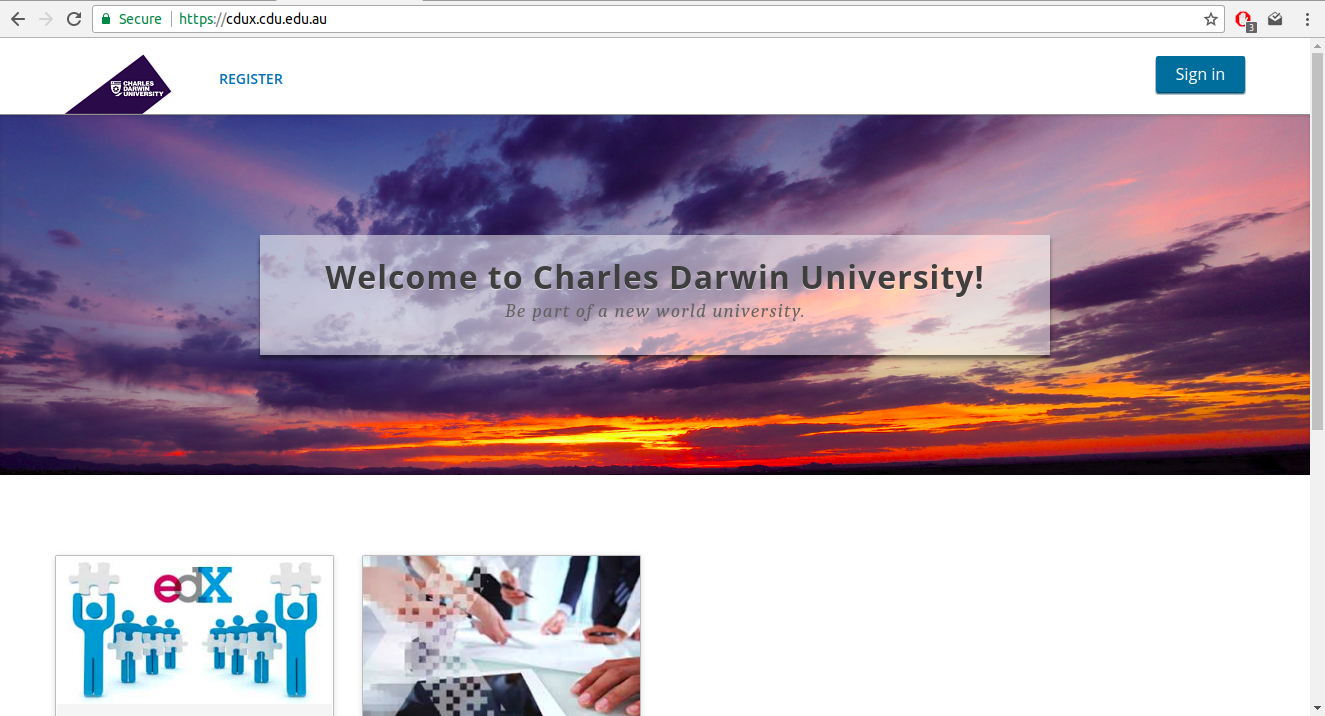
\includegraphics[scale=0.25]{lms}}
\caption{The landing page of the LMS.}
\end{figure}
\hspace{1.5cm}
\begin{figure}[h]
\centering
\fbox{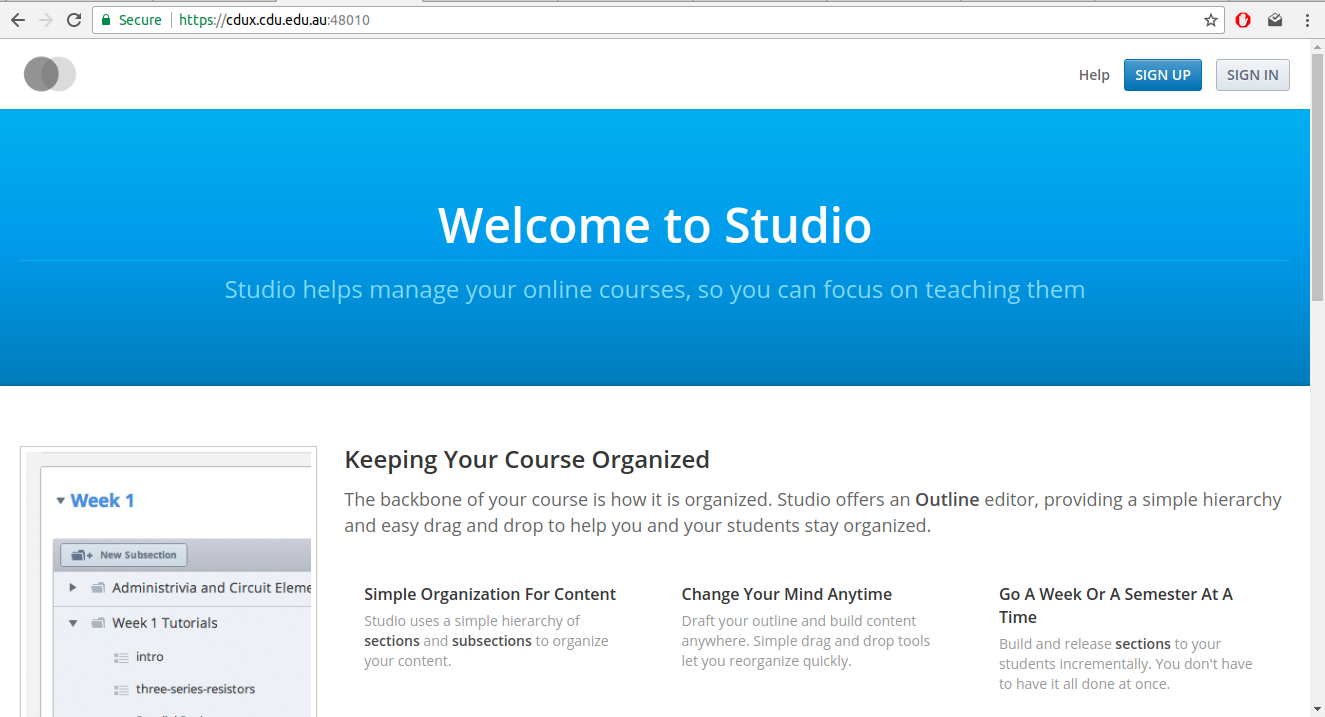
\includegraphics[scale=0.25]{studio}}
\caption{The landing page for the studio.}
\end{figure}

\subsubsection{Pedagogy}
In recent times, it has become apparent MOOCs have not brought about the democratisation in higher education widely purported by media outlets in 2012 and 2013 (NEED REFERENCE HERE). Moreover, XXXX (XXXX) suggest that MOOCs may have had a negative effect on aspects of higher education, momentarily diverting the attention of executive talent away from more important concerns. In light of this, care must be taken not to be dismissive of the eLearning findings borne from increased focus on MOOCs. The wealth of newly captured data has provided many opportunities for meaningful exploration. Much of the pedagogy, on which this introductory offering of PRT551 is based, has been founded on some of these findings.\\

One area in which interesting research has been undertaken, is in the phenomenon of mind wandering with respect to online settings. Mind wandering, in traditional classroom environments, has been widely researched and found to occur in lectures after approximately 10 - 15 minutes, resulting in poorer performance XXXXX.To counteract these findings, most higher education providers recommend teachers interleave lectures with tasks designed to supplement learning and re-focus student attention (Myers \& Jones, 1993). Often this is referred to as \textit{interpolated testing}. Not surprisingly, these findings have been replicated in the online setting too. In a review of recent studies on mind wandering in online settings, Szpunar, Moulton, and Schacter (2013) concluded interpolated testing can simultaneously reduces mind wandering, and increases task-related activities such as note taking. The content structure on CDUX, for PRT551, is organised to take advantage of interpolated testing. Students are made aware that there will be exercises interspersed throughout the lecture content, and are encourage to take notes which will aid them in negotiating these sections of the course.\\

In order to accommodate the interpolated testing structure, videos of 6-9 minutes in length were used. Of course interpolated testing could be just as easily accommodated using lectures of 20 to 30 minutes in duration - why choose 6-9 minutes? A study conducted by the MIT Computer Science \& Artificial Intelligence Lab, in 2014, found that student engagement peaked in the 6-9 minute category, with longer durations resulting in falls of normalised median engagement. This can be seen in Figure 6, which was taken from the study. In addition to recommendations on length, the study made a number of other recommendations, which are summarised in Table 4. The recommendation to use Khan-Academy style lectures was adopted by utilising a software package allowing the user to write fluidly on .pdf documents. The subject material for PRT551 did not lend itself naturally to this style of lecturing, however, this was partially overcome by simply marking up the slide as the lecture progressed. One final recommendation taken from the report was to record in a low cost setting instead of a professional studio was adopted, however, it must be noted that this recommendation was adopted more so out of budget constraints, and lack of access to professional studio resources.\\

Kearsley (2000) suggests that the virtual classroom is a `unique social context, much different to that of a regular classroom'

The benefits of Peer Instruction (PI) ...
Talk about the use of MOOC discussion forums, but then provide evidence that the use of these is not particularly widespread. Then talk about the 

Arguement

Students who are undertaking distance education are disadvantaged because of the lack of face to face social interaction with their peers. (Need reference) Although not all students take advantage of this. (Need reference)

Discussion forum is used tp encourage interaction among peers in the course. Discussion forums are set up according to these following procedures which are advised by this article (Need reference). This type of interaction is limited in its benefits according to (Need reference here). The core element that students learn in these modes is the interpretation of the expression of other students ideas - given that the Discussion forums are some what under utilised, peer assessments are used. Peer assessments get students to read the expression of other students ideas and provide a grade according to a rubric, and some model answers (is this beneficial - Needs References).

\begin{figure}[h]
\centering
\frame{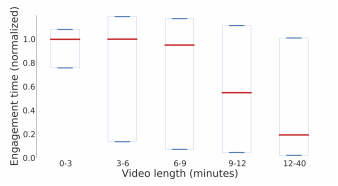
\includegraphics[scale=0.8]{engagement}}
\caption{A boxplot of engagement time normalised to each video's length. In each box, the middle red bar is the median; the top and bottom blue bars are the 25th and 75th percentiles, respectively. The figure was taken from Guo, Kim, \& Rubin (2014).}
\end{figure}

\begin{table}[h]
\centering
\caption{Summary of the main findings and video production recommendations, according to Guo, Kim, \& Rubin (2014).}
\scalebox{0.8}{
\begin{tabular}{p{7.5cm} p{7.5cm}}
\toprule
\textbf{Finding} & \textbf{Recommendation}\\
\midrule
Shorter videos are much more engaging. & Invest heavily in pre-production lesson planning to segment videos into chunks shorter than 6 minutes.\\
 & \\
Videos that intersperse an instructor's talking head with slides are more engaging than slides alone. & Invest in post-production editing to display the instructor's head at opportune times in the video.\\
 & \\
Kahn-style tablet drawing tutorials are more engaging than PowerPoint slides or code screencasts .& Introduce motion and continuous flow into tutorials, along with extemporaneous speaking.\\
 & \\
High quality pre-recorded classroom lectures are not as engaging when chopped up for a MOOC. & If the use of pre-recorded classroom lectures are a must, then instructors should plan with the MOOC format in mind.\\
 & \\
Videos where instructors speak fairly fast and with high enthusiasm are more engaging. & Coach instructors to bring out enthusiasm and reassure that they do not need to purposely slow down.\\
 & \\
Students engage differently with lecture and tutorial videos. & For lectures, focus more on the first-watch experience; for tutorials, add support for rewatching and skimming.\\
\bottomrule
\end{tabular}
}
\end{table}


\subsubsection{Lecture Slides}
Lecture slides were created using Latex. A simple design was used and the full course assets for the slides can be found on Github for download at the following link:\\
\begin{center}
\verb|https://github.com/skreynolds/PRT551_projectmanagement.git|
\end{center}

\subsubsection{Lecture Vidoes}
Lecture videos were created over the course of approximately 3 months. The final format for the lecture videos was faceless lecture slides, which were marked up in real time with an accompanying vocal overlay. The content creator for the videos was not a subject matter expert in Project Management, which caused a number of delays in producing a satisfactory product. The main technique used to aid in the production was to record lecture videos in a piecemeal, discontinuous fashion. This allowed concise, accurate statements to be made and then stitched together using a post production software environment. Camtasia was the main software used to capture and edit video assets. A program called PDF Annotate was used to mark up the lecture slides. The hardware used to produce the content was selected because it was cheap, reliable, and available. The tablet hardware used was an ATIV, shown in Figure XXX. The microphone used was an Audio technica, shown in Figure XXXX.

\begin{figure}[h]
\begin{minipage}{0.45\textwidth}
\centering

\includegraphics[height=100px]{ativ}
\caption{text}
\end{minipage}
\hspace{1cm}
\begin{minipage}{0.45\textwidth}
\centering

\includegraphics[height=100px]{microphone}
\caption{text}
\end{minipage}
\end{figure}

\subsubsection{Lecture Activities}
Lecture activities were used principally to implement interpolated testing, which was discussed in Section 4..1 of this report. Basically, interpolated learning requires short bursts of theory, punctuated by activities which require the learner to access recently learned knowledge and apply it in rudimentary questions. With this in mind, a series of activities have been created. The following formats were used:
\begin{itemize}
\item Multiple choice
\item Check box
\item Numerical entry
\item Informational sorting questions
\end{itemize}
Why is this good? What other questions could be used. Put a statement that this is for proof of concept only.
Students can answer these questions as many times as they like to get the correct answer, unlike the tutorial questions on which students only have one try to get the questions correct.

\subsubsection{Tutorials}
Tutorials sit are the end of each week and are composed of approximately 5 questions each. They types of questions that are used are:
\begin{itemize}
\item Multiple choice
\item Short answer questions
\end{itemize}
The interesting part here is the use of the short answer questions. Each question requires the student to enter a paragraph or so to answer a question which is posed. Given that it would be resource intensive to get CDU staff to mark the individual repsonses - this has been instead set up as a peer review activity. Rubrics have been provided to students and each student response goes to two other students for review. Note that in order for this to work properly, we need a multiple of three students present in the course assuming that every student participates in the short answer questions. 

At the time of writing this, this feature has yet to be tested.

\subsubsection{Case Study}
The case study was included to provide a PASS FAIL grade for the course. The task was a simple case study that students had to create a mind map and a couple of other bits and pieces which were really ill defined. In the event that the platform is used for marketing to overseas students, then they may be able to get some basic credit for the platform.

\section{Potential Uses for CDUX}
Given that the commerical LMS that CDU uses is Blackboard, and the fact that managing onsite software carries a host of complications which goes against the economic theory of specialisation and trade. There are limited uses for the CDUX platform. Two of the hypothesised uses for the platform on campus could be:
\begin{itemize}
\item Using as a marketing tool for encouraging students to study with CDU
\item Hosting courses which students can access irrespective of their enrolment status
\end{itemize}

\subsection{Marketing Tool for Applicants to the CDU Masters of Engineering and IT}
Currently the School of Engineering at Charles Darwin University fields almost \textbf{XXXX} applications annually, for its postgraduate program Master of Engineering and Master of IT. The applications that are accepted by the University are approximately XXXX per annum, and approximately XXXX\% of these students convert to studying at CDU. Using CDUX to provide a free introduction to students considering studying at CDU may lead to a higher conversion of students to studying at CDU.

This is a seemingly tenuous marketing strategy, however, there is evidence to support in the following paper XXXXX where shows evidence of increased conversion of applicaotins to paying students.  

What would this look like for for university to host something like this and what would be the protocols for managing the platform et cetera

At this stage without further ratification of the materials this remains a curiosity, rather than an actual marketing strategy.

\subsection{Platform to host short courses produced by ALLSP and other Student Support Services}
There is some difficulty in using Blackboard/Learnline to create courses which are offered to students which aren't for credit. There are many products on the market which allow the creatioin of courses, however, the underlying software is not controlled by the university and these courses may be accessed by students from outside the university (this is not really a problem though, and creating courses on this type of platform which are not for credit may even raise CDU's profile by providing entry level marketing). Why this platform? no real reason for undertaking this - principal benefits are that the university can restrict the participants that are using the platform

\section{Cost}
A single 50 hour contract at tutor rates, though it must be noted that significant time was spent developing the course material, including filming the video lecture assets. Additional costs are the ITMS labour and assets, and the meeting time from the group that helped to provide the guidance for the project.

\begin{table}
\centering
\caption{text}
\begin{tabular}{lr}
\toprule
\textbf{Item} & \textbf{Cost}\\
\midrule
\bottomrule
\end{tabular}
\end{table}

\section{Concluding Remarks}

\section{References}
Activation Email

Thank you for signing up for CDUX.\\

Change your life and start learning today by activating your CDUX account. To activate your account please send an email to shane.reynolds@cdu.edu.au with the user name and email address you used to register this account.\\

If you didn't request this, you don't need to do anything; you won't receive any more email from us. 

Please do not reply to this e-mail.

If you require assistance, check the about section of the CDUX web site.

\end{document}